\NeedsTeXFormat{LaTeX2e}
\documentclass[10pt,a4]{scrartcl}

\usepackage{tabularx,longtable,graphicx,a4,listings,wrapfig,subfigure,textcomp,ccaption,latexsym,setspace,algorithm,algorithmic,esvect,color}
\usepackage[absolute]{textpos}

\ifx\pdfoutput\undefined
  % We're not running pdftex
  % european (better) fonts -- does not look good with pdflatex
  \usepackage[T1]{fontenc}
  \newcommand{\href}[2]{#2\\{\hspace*{5mm}\scriptsize <#1>}\\}
\else
  \pdfcompresslevel=9
  \def\pdfBorderAttrs{/Border [0 0 0] } % No border around Links
  \usepackage{hyperref}
\fi

\title{Project, Virtual Reality\\Group 8}
\author{Stefan Eilemann}

\newcommand{\tm}{\texttrademark~}
\newcommand{\rc}{\raise 1ex\hbox{{\tiny\textregistered}}~}
\newcommand{\fig}[1]{Figure~\ref{#1}}
\newcommand{\sref}[1]{Section~\ref{#1}}
\newcommand{\aref}[1]{Appendix~\ref{#1}}
\newcommand{\link}[1]{\htmladdnormallink{#1}{#1}}
\newcommand{\fix}[1]{\textbf{\color{red}{#1}}}
\indentcaption{2em}

% suppress  single floating lines on top (widow) and bottom(club)
%  10000 is infinity
%  tradeoff: maybe underfull vboxes
\clubpenalty=10000
\widowpenalty=10000
\date{Mar 20, 2013}

\begin{document}
\maketitle

\section{Project Description}

The project builds upon the Equalizer parallel rendering framework and one of
its example programs, eqPly. It adds the following features to either the
core framework, where it is generic, or to the application, where it is not:
\begin{itemize}
\item Render any 3D object in the ply file format on any display system
  supported by Equalizer (LCD, stereo screen, CAVE, display wall) using
  monoscopic and stereoscopic (active, passive and anaglyphic) rendering.
\item Generic, transparent head tracking in the core framework, based on
  OpenCV. The tracking will provide X,Y translation, an estimation of the
  observer's Z distance, and when possible, roll estimation using the eye
  positions.
\item Object manipulation using the Logitech 3D Spacemouse. The Spacemouse
  delivers relative sensor data for six degrees of freedom (rotation and
  translation), which will be used to move an object in the scene accordingly.
\item create a waterfall modeled using a particle system based on a physics
  library, which will flow around the displayed model. A spatial data structure
  is used to ply model the interaction between the model and the particle
  system.
\end{itemize}

\section{Tools and Methods}

The project is integrated into the Equalizer parallel rendering framework, where
possible in the core library. The non-generic parts of the work are build into
\textsf{eqPly}, the polygonal rendering example shipped with Equalizer. The
Equalizer programming and user guide has a detailed description on the structure
of \textsf{eqPly}

OpenCV is used for head tracking. The support of OpenCV is generic in Equalizer,
a new field configures the camera index used for each observer. The support is
conditional on the availability of the OpenCV library and headers at compile
time, as well as on the presence of a camera at runtime. A face and eye
detection filter continuously estimates the 3D position in space, and if eyes
are detected, the roll of the observer. Head and pitch are not estimated due to
the limited amount of freedom given by a single camera input. Since the computer
vision is computationally expensive, the OpenCV head tracker runs asynchronous
in a separate thread from the main application loop. After each detection, it
injects an observer event into Equalizer, which is processed by the normal event
handling flow.

For interaction, a 3D space mouse is used. This device reports relative values
for six degrees of freedom. Again, the spacemouse support is fully integrated
into the Equalizer event handling code, and the events are processed by
\textsf{eqPly} to manipulate the model matrix applying the six delta values in a
one-to-one mapping onto the model. Three different backend implementations
receive and convert the event from the device into a generic representation: a
\textsf{spnav} implementation for GLX (X11, Linux), an implementation based on
the official driver for AGL (Carbon, Mac OS X) and a raw message-based
implemenation for WGL (Windows).

%\fix{Physics:}

\section{Installation}

Since our project is embedded in a larger software, building it may be a bit
more complex. The build and functionality has been test on Mac OS X 10.8 using
the command line XCode utilities and MacPorts. Equalizer and all its
dependencies is build using the Buildyard multi-project CMake build tool, which
will download, configure, compile and install all projects in the correct
order. The only other dependencies to be installed are MacPort and the official
Mac OS X drivers for the SpaceMouse, and then the example can be build as
follows:

\begin{lstlisting}
sudo port install bullet +universal
sudo port install boost +universal
sudo port install opencv +universal
sudo port install cmake
cd Buildyard
make Equalizer
\end{lstlisting}

Afterwards everything is installed in \textsf{Build}, and the \textsf{eqPly}
example application can be launched:

\begin{lstlisting}
./Build/Equalizer/bin/eqPly.app/Contents/MacOS/eqPly
\end{lstlisting}

\section{Discussion}

This project contributed new functionality into an existing open source
project. While this added additional requirements to the project, this work
immediately benefits the existing users of the Equalizer parallel rendering
framework. Furthermore, building unto an existing framework also facilitates the
implementation due to the reuse of existing infrastructure and functionality,
e.g., the already-build rendering application. The resulting demo is rich in
features and can easily be deployed on virtually all types of display systems.

\begin{wrapfigure}{r}{.312\textwidth}
  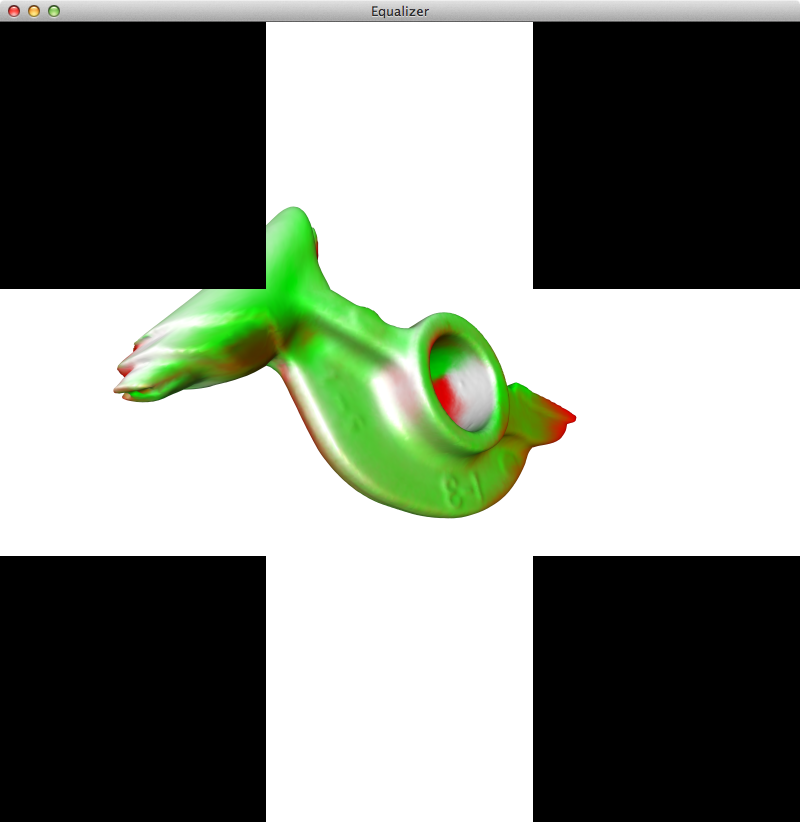
\includegraphics[width=.312\textwidth]{screenshot}
  {\caption{\label{fScreenshot}eqPly running in a five-sided cave emulation}}
\end{wrapfigure}
Due to the previous knowledge with Equalizer, the integration of the spacemouse
and OpenCV was relatively straightforward. The correct design of integrating
camera-based tracking took some time to figure o out. At first, a synchronous
approach polling the camera each frame was used, where the actual detection was
used to another thread. This proved too complex and hard to integrate cleanly
into the existing design, which was finally solved by an asynchronous approach
injecting events into the already distributed event processing. The chosen
design is simple in its implementation and robust in execution.

\end{document}
